\documentclass[twocolumn]{article}

\usepackage[letterpaper,margin=1in]{geometry}
\usepackage{url}
% \usepackage{times}
\usepackage{graphicx}
\usepackage{fullpage}
\usepackage{indentfirst}
\usepackage{fixltx2e}
\usepackage{hyperref}
\usepackage[font=small,labelfont=bf]{caption}

% \usepackage{setspace}
% \setstretch{1.1}

% \setlength{\parindent}{0pt}
\setlength{\parskip}{1.5ex}
\setlength{\columnsep}{1em}


\begin{document}

\title{Using Twitter and MapReduce to Predict the Stock Market}
\author{Marcus Gartner \and Tala Huhe}
\date{Final Project - CSCI 2950-U - Fall 2011}
\maketitle

\begin{abstract}
\noindent
It has been proven that user created data on Twitter, called Tweets, can predict the stock market \cite{bollen}. The approach used is one that is inherently biased because it measures the correlation between stock price and the general “mood” of a sample of Tweets based on predetermined mood indicating terms, making assumptions about language and the use of language. In addition, previous work done on this topic provides no insight into the implementation required to be useful in a real-world trading environment in which predictions must be made in a timely fashion.

In this paper we show an implementation of a distributed application which attempts to provide an unbiased prediction of the stock market using data from Twitter. We also evaluate the runtime requirements of the application in order to show its effectiveness for use in a real-world environment. Our application is able to make predictions of the percent change in the price per share of an aggregation of several stocks within X\% of the actual value Y\% of the time.
\end{abstract}

\section{Introduction/Motivation}
Twitter is a social application that allows users to post messages, called tweets, which can be read by their friends or the general public. Twitter’s 300+ million users tweet millions of messages per day creating a huge amount of data. The information contained in this data has been shown to have a strong correlation with the stock market and used to predict the value of stocks in the future \cite{bollen}. Our goal is to build upon this concept by attempting to make predictions using a different method, while also tackling the challenge of processing the large amount of data in an efficient way.

We attempt to improve upon the method used in \cite{bollen} to predict the stock market with Twitter by creating a less bias algorithm. The method used by Bollen et al. is slightly convoluted in that it adds an unnecessary layer of abstraction. They first determine the “mood” of Twitter during a time period, or sample, by analyzing tweets based on mood phrases, for example, “I feel happy”. Once they create this abstraction they use the mood index of a time period to predict how the market will behave. This solution is biased because it makes assumption on the use of language and the meaning of the “mood words”. It also creates an unnecessary direction of abstraction.

Our algorithm is able to relate Tweets directly to stock prices. We adopt the vector space model from information retrieval to determine a tweet sample’s similarity to other tweet samples that have been previously recorded. Then we create a prediction of the stock market by analyzing the market’s behavior during these similar historic time periods.

We utilized a number of Amazon Web Services to collect, store and process our data, namely, Elastic Cloud Compute (EC2) instances, Simple Storage Service (S3), SimpleDB (SDB), and Elastic MapReduce (EMR).

\section{Prediction Algorithm}
A prediction of the market is generated by first finding the most similar historic Twitter samples, then averaging the percent change in price per share of stocks of the time periods corresponding to these samples. The prediction is in the form percent change in price per share. In effect, what we are doing is finding periods of time in the past when publicly posted tweets have similar content to the current period. The prediction is then created on the assumption that the stock market with behave similarly as it during those similar periods.

To find the most similar historic Twitter samples, we use an algorithm based on the vector-space model that has been used extensively by web search companies. The algorithm has been altered to fit our needs. Specifically, the common web search query-document based algorithm is designed for matching queries, usually of length less than ten, to documents with thousands of words. Therefore, adjustments had to be made to make the algorithm more suited for comparing two samples both containing hundreds of thousands of words.

$$ Score(s_1, s_2) = \frac{\sum_{t \in s_1 \cap s_2} 2+tf_{s_1}+tf_{s_2}}{(m_{s_1}+m_{s_2}) / m_{max}} $$ 	

The similarity of two samples is the total number of occurrences of all common words between $s_1$ and $s_2$ divided by the quotient of the sum of the number of words in $s_1$ and $s_2$ over the size of the biggest sample. We add up the occurrences of common words on the assumption that the more words samples share, the more similar they are. This sum is divided by the ratio of the sample sizes to the max sample size to normalize the score. We must normalize these scores based on sample size because the number of tweets can vary widely over the course of a day, varying the number of words in a sample. Without this normalization the largest samples would always have the highest similarity scores.

The prediction of the market can be trivially generated once we have determined the most similar samples. In order to generate a prediction for one particular hour, we examine the Twitter data that we have collected for the previous hour. We then find the hours in history with Twitter data that most resembles what we have collected. For each of the similar hours, we examine the relative stock change over the succeeding hour and average the percent changes in price per share together to determine our prediction.

\section{Data Collection}
Our algorithm relies on having a historical collection of twitter data. To collect this data, we utilized Twitter’s Streaming API which, at the free tier, provides a random stream of tweets in real-time that constituted approximately 1-2\% of all tweets. We used a virtual server, an EC2 instance, to pull tweets via the Streaming API and upload them in hourly increments to S3. Note that we made our sample time period one hour long, but any sample time period could be used.

We pulled approximately 4.5 GB worth of raw tweets per day, accumulating over 400 GB of data during the three month period in which we were collecting data. 

The stock data was more challenging to collect. Unable to find a good source of free intraday stock data, we wrote a scraper over the Yahoo! Finance API. This REST API allowed us to collect data on an incremental basis. We ran a periodic script on an EC2 instance to fetch Yahoo! stock data and upload it to SDB for storage on an hourly basis. Our scraper collected all of the data Yahoo!’s API offers on several chosen tickers. We collected stock data for the Dow Jones Industrial Average, NASDAQ Composite, NASDAQ USA, NASDAQ-100, Apple, Sony, Johnson-and-Johnson, and Microsoft. We believe this data is a fair representation of the market.

\section{Implementation}
In practice, we implemented a three step process in which a prediction is created. First the raw twitter data is preprocessed and an index is built for easy access to information regarding each sample. Then a comparison step scans through the index and for a given sample outputs the similarity score of each sample in the index. With this list of similarity scores, a prediction can be made by looking up the historical stock data associated with the most similar samples.

\subsection{Building the Index}
The preprocess step analyzes each raw tweet and for an hourly sample produces a list of each word that appears in the sample and the number of times it appears. The data received from the twitter represents each tweet as a JSON object which contains the tweet text, along with metadata about the user who posted the tweet and the tweet itself \cite{twitterget}. For our use we were only concerned with the text of the tweet and the time the tweet was posted. 

Once this data was parsed out, we further massaged the text of the tweet. First, we filtered out tweets that were not in English. We used the Ruby WhatLanguage library which is able to determine between several different languages and calculate the most likely language a sample of text is written in \cite{whatlanguage}. The next step was to filter out stop words from the text of each tweet. Stop words refer to words that are so common that they provide no added value in determining the similarity score of two samples. Our list of 39 stop words included terms such as “a”, “an”, “are”, and “the”. 

One further process we performed on the text of each tweet was stemming. Stemming removes common suffixes of related words so that the scoring algorithm treats these words as the same word. For example, “productive”, “productively”, and “productivity” all stem to “product”. Stemming each word in the text produces better similarity scores and reduces the size of the index being created. We were able to use the PorterStemmer library which is available in a number of programming languages \cite{porterstem}. Note that the primary reasons for filtering out non-English tweets was because this simplifies the list of stop words and because the stemming library we used is only able to stem English words.

We implemented our index builder in Ruby and ran it using the Hadoop streaming feature of EMR. Hadoop Streaming reads a collection of input files from S3 and passes each line of the files to the standard input of a mapper function. The mapper then prints each output tuple to standard output which Hadoop Streaming sorts, and passes to the standard input of a reducer function. The output of the reducers is written back to S3. Hadoop streaming provided us the ability to write our mapper and reducer functions in simple Ruby scripts, thereby reducing development time.

The mapper for the build index step reads each tweet, parses the JSON object, filters out non-English tweets, excludes stop words, and stems the remaining words as described above. The mapper then outputs tuples in the form \texttt{<timestamp, word\textsubscript{i}, 1>} for each word, where timestamp is the hour in which the tweet was posted. The reducer function aggregates the words for each hour sample, adds up the occurrences of each word, and outputs a list for each sample period containing each word in the sample and the number of times it appears.

\subsection{Finding Similar Samples}
To find the most similar samples to a given sample, $s_1$, we compute the similarity score of the given sample paired with each historical sample. We ported our similarity algorithm to the MapReduce paradigm again utilizing the benefits of Hadoop Streaming running on EMR. The mapper function of this step takes as input each indexed sample in the previously constructed index that is stored in S3. For each historic sample, $s_2$, it adds up the counts of the words that $s_1$ and $s_2$ have in common, creating a temporary score. It outputs tuples in the form \texttt{<ID\textsubscript{s\textsubscript{2}}, temp\_score, size\textsubscript{s\textsubscript{1}}, size\textsubscript{s\textsubscript{2}}>}. Then, a single reducer reads each tuple from every mapper, and calculates the final score by performing the normalization step, where each temporary score is divided by the relative size of the two samples. The reducer orders the samples by score, and writes a file to S3 containing the results.

\subsection{Generating a Prediction}

\begin{figure*}
\centering
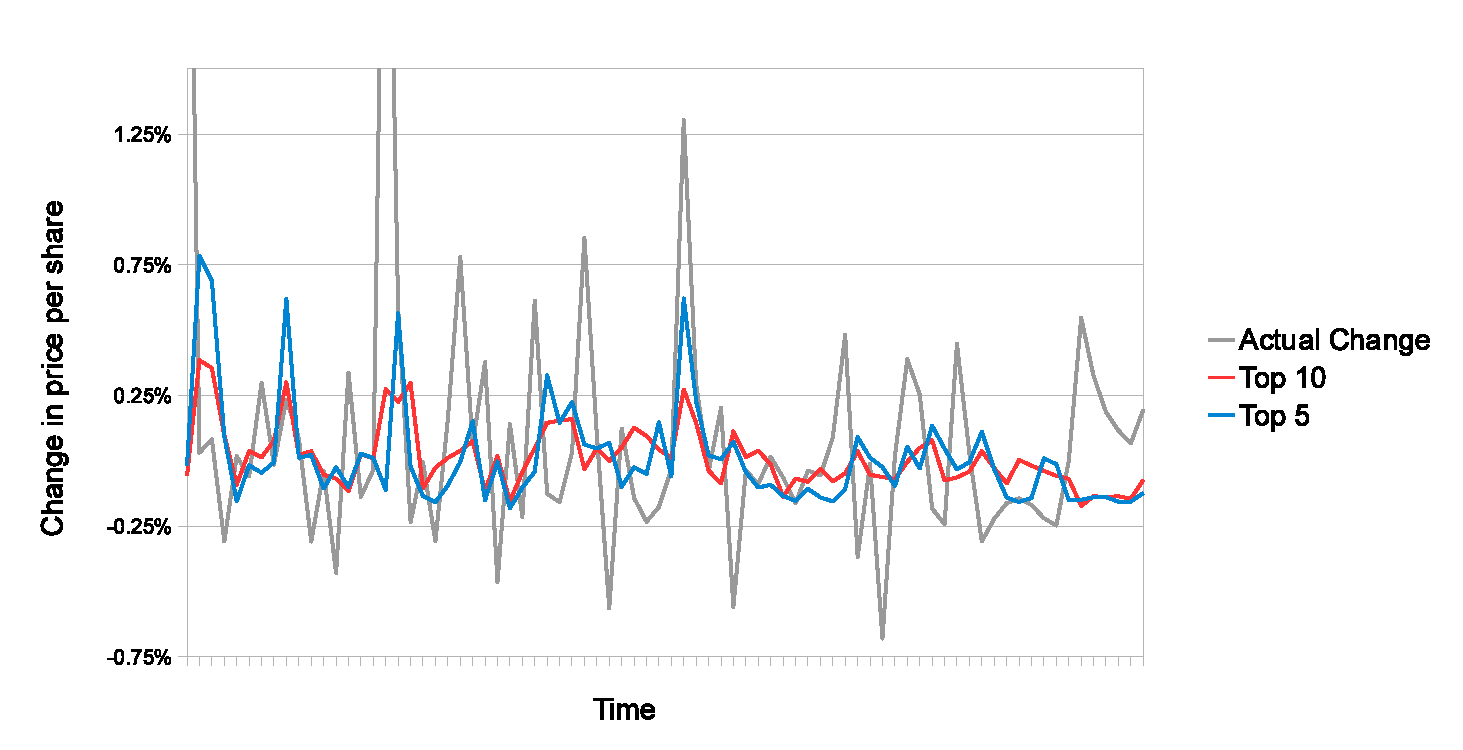
\includegraphics[width=1.0\textwidth]{predictions}
\caption{Predictions generated between 9:00 am, Nov. 28, 2011 and 2:00 pm, Dec. 9, 2011 during market hours using both the top 5 and top 10 most similar Twitter samples.}
\label{predictions}
\end{figure*}

When we plotted our scraped data, we discovered that Yahoo! Finance API did not provide us with accurate data. First, we were unable to collect data on off-hours changes. This lead to large flatlines in weekend areas. Second, Yahoo! Finance API sometimes failed to provide us with ticker data that we had asked for. Third, the API provided us with incorrect data. We ended up discarding Johnson and Johnson stock data as a result. Fourth, the API was inconsistent about its ticker usage. Approximately halfway through our data collection phase, Yahoo! started using a different symbol for the NASDAQ Composite ticker. Finally, the API was inconsistent about its data fields. For non-aggregate tickers, asking and bidding price seemed to work; however, for aggregate tickers, these values were always N/A.

In order to combat these problems and sanitize the data we devised a three-step process. First, we identified symbol changes and migrated all data pertaining to a particular ticker to a consistent symbol. Second, we created a consistent data field which we used to store the most recent stock price. For non-aggregate tickers, we were able to use an average of real-time asking and bidding price; for aggregate tickers, we used the last trade price. Lastly, we filled in the missing data points using linear interpolation. This was necessary to avoid throwing away a good chunk of usable Twitter data.

After the three-step sanitization process, we computed the hourly changes and relative hourly changes (percentage) between all of our data points. This was a fairly simple step after sanitization.

Generating a predicted percent change in price per share of a stock is done by utilizing the most similar samples for each time period. For a given timestamp $t$, we start by fetching the most similar timestamps $sim_t$ generated by the algorithm above from S3. The prediction is created by computing the average change in price per share of a stock over the next hour. 

We found that by average a large number of samples our predictions approached zero. This is likely due to the law of large numbers. Since the average prediction will indicate no change, averaging a large number of predictions, even over similar hours, will cause the result to be very close to no change. We found that using any more than 25 results caused the predictions to be too close to zero for comparison. This means that we needed to severely limit the number of results to obtain a semi-accurate prediction. Some of the methods we used included using only the most common hour, using the top X hours, using hours with similarity above Y, and using the top Z\% most similar hours. Using only the most common hour resulted in too much statistical noise. Thresholding similarity via a constant caused a variety of problems, since the range of similarity scores were different for each hour. We also tried a dynamic threshold, but found that it performed slightly poorer than simply using the top X documents. We found that using the top 5, 10, and 15 documents seemed to produce the most consistent and accurate results.

We also tried a variety of schemes to weight the stock changes with respect to the similarity score between samples. However, since all of the top hours were similar in nature, the similarity scores differed only slightly. This meant that using linear weights altered the final prediction minutely compared to weighting each top sample the same. 

We also used a variety of aggregation schemes to combine results across all of our stock tickers. We initially began by only using the NASDAQ. However, due to the flakiness of our stock data and the general instability of using one ticker, we obtained poor prediction results. We then compared using an average of all of the aggregate tickers versus using an average of all of the corporate tickers. Though the two were similar, we found that the aggregrate tickers generally produced more stable data points. Our final results are generated with the Dow Jones Industrial Average and NASDAQ.

Our prediction generation codebase is written in Python and uses Boto, a Python library for accessing Amazon Web Services programatically. We have one large script written for sanitizing the Yahoo! data as outlined above. We have an additional script for computing differences, and finally one for generating predictions based on those predictions. 

\section{Evaluation}

\begin{figure}
\centering
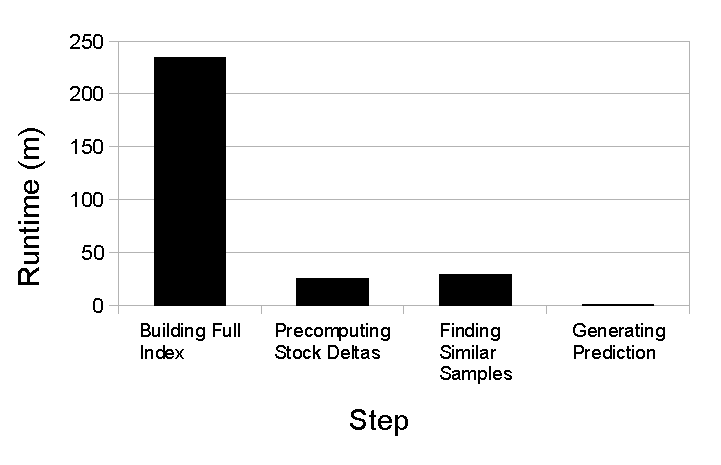
\includegraphics[width=0.5\textwidth]{runtime}
\caption{Runtime in minutes of each step in the process of generating a prediction. Building the full index was executed on a cluster of 19 virtual machines, and finding similar samples was performed on a cluster of 4.}
\label{runtime}
\end{figure}

Evaluation of the runtime of each step in the process shows that building the historical index is the most time consuming step. As seen in figure \ref{runtime}, this step took 234 minutes on a cluster of 19 virtual machines to build an index for three months of Twitter data. While we built the entire index in one execution, our system could be altered to build the index incrementally as new tweets are collected in real-time, therefore eliminating the need to build the entire index each time new samples are added.

The step which finds the most similar samples for a given sample took on average 28.7 minutes on a cluster of 4 virtual machines. The other two steps, precomputing the change in stock values for each hour which took on average 25 minutes, and generating a predicted percent change in stock price given the most similar historic samples which took less than 1 minute, both ran on a single machine.

\begin{figure}
\centering
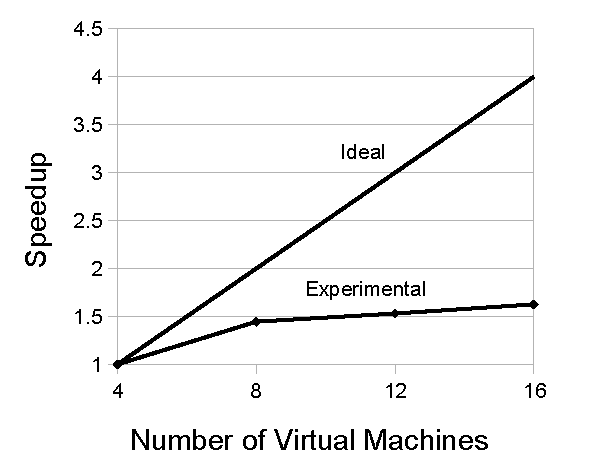
\includegraphics[width=0.5\textwidth]{speedup}
\caption{Scalability of finding similar samples for a given hour sample. It scales rather poorly because the application uses a single reducer which is a major bottleneck.}
\label{speedup}
\end{figure}

We examined the experimental scalability of the step in the process in which the most similar historic samples to a given sample are found. We focused on this step because in practice this step would be executed more frequently than the step which builds the full index, and because generating predictions once similar samples are found occurs on the order of tens of seconds on a single machine, which is fast enough to be considered relatively instantaneous. The results showed very poor scalability with a speedup of 1.44 with 8 virtual machines, 1.53 with 12 virtual machines, and only 1.63 with 16 virtual machines, as seen in figure \ref{speedup}. This speedup is far less than ideal because of the bottleneck from using only one reducer.

\begin{figure*}
\centering
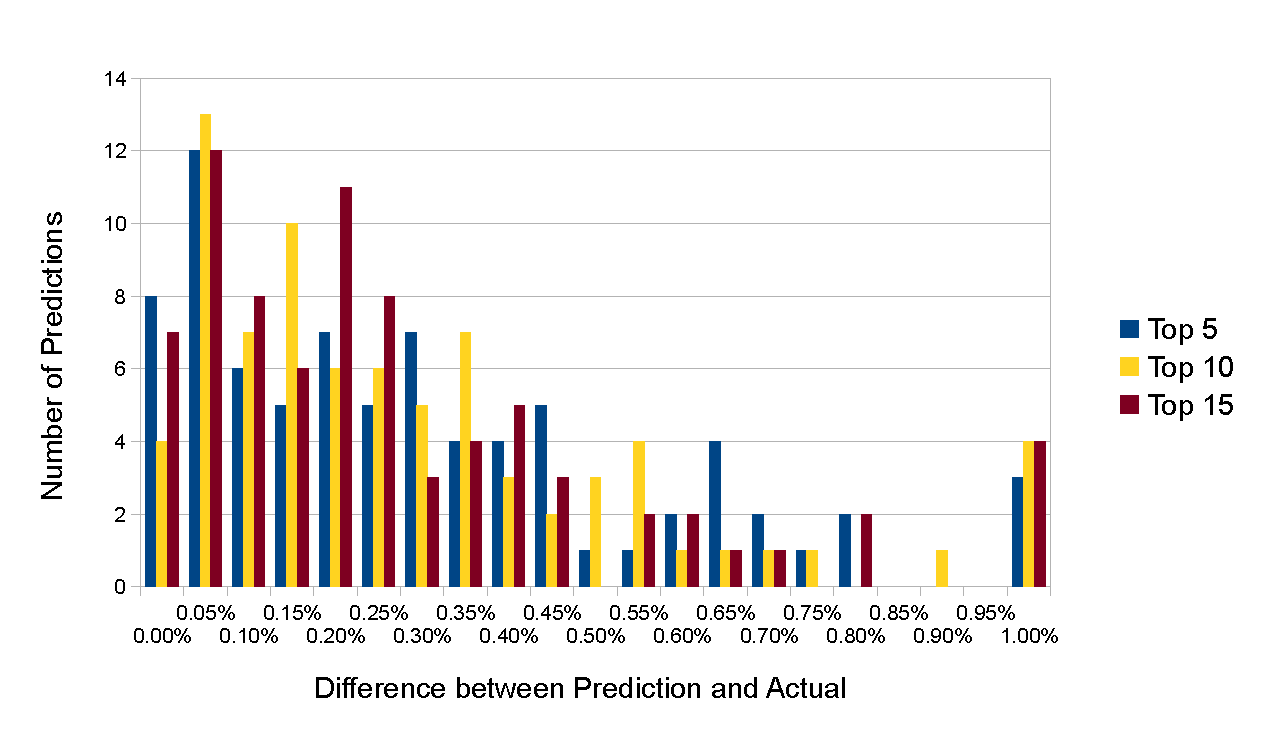
\includegraphics[width=0.9\textwidth]{histogram}
\caption{Histogram of the difference between our computed prediction and the actual percentage change over all aggregate stock symbols. The three different data sets correspond to using the top 5, 10, and 15 most similar samples to generate the prediction, respectively.}
\label{histogram}
\end{figure*}

Given the runtime required to find similar Twitter samples, and the application’s poor scalability, this system is not feasible to use in a real-world scenario where a trader’s decisions would be based off of the system’s predictions. As the size of the historical data grows, the number of samples to score a specific sample with would grow, and the runtime of finding similar samples would increase. It is not hard to imagine this system taking longer than one hour to generate a prediction based upon one or two year’s worth of historic data, meaning that the prediction is worthless as the hour being predicted has already come and gone.

Our predictions were somewhat accurate overall. It is apparent to us that there is some sort of statistical correlation between similar tweets and stock changes; however, we lack the data to sufficiently prove this relationship and demonstrate that it would be useful to a trader. We found that the majority of our predictions were very close to the actual stock changes, as evidenced in figure \ref{histogram}. Using the top 15 most similar samples, 32.00\% of the predictions were within 0.1\% of the actual change. In addition, 69.33\% of the predictions were within 0.25 of the actual change. In fact, most of the time our result matched the sign of the actual change. However, due to our weak data, we are unable to generate a more meaningful result. 

\section{Future Work}
Ideally we would have evaluated the accuracy of our predictions using a longer history than 3 months. This was not possible over the course of the semester, but it would be interesting to see how our prediction accuracy changes with a bigger history to formulate predictions on. As the size of the increases, the run time of making the prediction also increases. If too long of a history is used, making a prediction using our current implementation might be impossible to do in a timely manner. Older Twitter samples could be grouped together by similarity along with the corresponding stock data in a preprocessing step. This would reduce the number of sample pairs scored when generating a prediction, thereby reducing the run time required to make a prediction.

In our implementation we built the entire index once we had collected all of our data. This makes the system not a real-time system. To make the system practical in a real-world setting where generating predictions would need to happen as fast as possible the full index would have to be built incrementally. As new tweets are received from the Streaming API, a distributed queue system could managed unprocessed tweets. Worker machines could pull tweets from the queue to preprocess and add to the index.

An additional improvement to our system would be to keep track of the largest sample size (measured by number of words in the sample) in the full historic index. This would remove the requirement of using a single reducer in the step of the process which finds similar samples. Without this bottleneck, the scalability of this step would Our goals were to present an algorithm for predicting the stock market based on public Twitter data which is unbiased and without unnecessary abstraction, and to provide the implementation of an application based on this algorithm. Our algorithm was able to predict . More work is required to verify whether our prediction algorithm could be beneficial in making trading decisions. More Twitter and stock data, and further analysis of computed predictions would prove or disprove the usefulness of our proposed algorithm.

The application we built was shown to be impractical in a real-world trading environment. The lack of scalability of a step in our process pipeline which finds similar periods of Twitter content is a bottleneck that prevents our application from being useful in the real world. However, several aforementioned changes to our design could eliminate this bottleneck.greatly improve.

Bollen et al. are able to find correlation between their abstraction of the general mood of Twitter posts and the stock market in which the twitter mood is predictive of stock market behavior 3 to 4 days in advance. It would be interesting to build upon our system to evaluate the correlation of our predictions at any number of hours or days in advance. This would reveal how far in advance Twitter content shows clues of stock market behavior.

\section{Related Work}
The concept of correlating Twitter data to stock market behavior in such a way as to be able to predict market changes ahead of time was motivated by the work of Bollen et al. in \cite{bollen}. Our algorithm differs in that it attempts to link Twitter data directly to market behavior without creating an abstracted layer by calculating the mood of tweets. This allows us to not have to worry about the underlying meaning of the Twitter content. We do not have to make assumptions about the definitive or slang meanings of words.

Our algorithm builds upon common practices in information retrieval and web search. The vector-space model allows us to find the similarity between samples without having to reason about the underlying meaning of the words and language used in each individual tweet. Our final sample scoring algorithm differs slightly from the canonical query-document relevance ranking algorithm in web search. We altered it to produce better results when scoring two samples each with hundreds of thousands of words, as opposed to scoring a query of several words to a documents with thousands of words.

\section{Conclusion}
Our goals were to present an algorithm for predicting the stock market based on public Twitter data which is unbiased and without unnecessary abstraction, and to provide the implementation of an application based on this algorithm. Our algorithm was able to predict . More work is required to verify whether our prediction algorithm could be beneficial in making trading decisions. More Twitter and stock data, and further analysis of computed predictions would prove or disprove the usefulness of our proposed algorithm.

The application we built was shown to be impractical in a real-world trading environment. The lack of scalability of a step in our process pipeline which finds similar periods of Twitter content is a bottleneck that prevents our application from being useful in the real world. However, several aforementioned changes to our design could eliminate this bottleneck.

\bibliographystyle{unsrt}
\bibliography{writeup}

\end{document}

